
\section{Mécanique de la fracture linéaire élastique}
\label{sec:LEFM}

Nous avons présenté dans la section précédente qu'une interface frictionnelle entre deux solides possède une structure complexe, étudiée au travers de modèles empiriques macroscopiques, justifiés par des considérations microscopiques. Ces modèles comme celui de Bowden et Tabor ou de Dieterich et Ruina font état de la réalité des contacts microscopiques à l'interface, mettant notamment en évidence la différence entre l' entre l'aire de contact réelle $A_r$ et l'aire de contact macroscopique $A$ aire de contact réelle $A_r$ et l'aire de contact macroscopique $A$ entre les deux solides. Ils ne fournissent cependant qu'un modèle pour le déplacement moyen des blocs à l'interface. 
%sur l'approximation que les solides en contact se déplacent %d'un bloc, sans déformations internes, comme infiniment rigides.
L'élasticité responsable de leur mouvement de stick-slip est alors extérieure au système, modélisable par un ressort effectif relié à une masse indéformable en frottement sur une surface fixe.
Dans la réalité pourtant l'élasticité provient des blocs en frottement eux-mêmes. Ils sont élastiques et se déforment, y compris à proximité de l'interface. Le changement brutal de vitesse lors d'une phase de slip n'est en réalité pas instantané. Tous les microcontacts n'entrent pas en glissement simultanément, mais s'affaiblissent de proche en proche au cours d'un phénomène propagatif, un \textit{crack} ou \textit{fracture}, ou encore \textit{rupture}.

La propagation de cette fracture s'accompagne de la libération dans le matériau d'ondes de compression et de cisaillement se propageant jusqu'en surface, et qui dans le cas des failles sismiques donnent naissance à un séisme. Cette rupture engendre une chute de contrainte cisaillante locale, et se déplace à des vitesses pouvant atteindre la vitesse du son dans le milieu. Elle correspond à une fracture en mode de cisaillement, décrite par la mécanique de la fracture linéaire élastique (LEFM, pour \textit{Linear Elastic Fracture Mechanics})\,\cite{svetlizky_brittle_2019}.


Dans cette section, nous présentons les principes de la propagation de fractures dans les matériaux et leur application à l'étude des frottements solides. La première partie décrit les bases de la théorie de l'élasticité que nous allons utiliser par la suite, la deuxième les fondements de la fracture statique puis dynamique, dont la théorie de Griffith, et la troisième l'application de la mécanique de la fracture linéaire élastique à la propagation de ruptures le long des interfaces frictionnelles.





\subsection{Mécanique du solide élastique}
\label{sec:hook}
La mécanique du solide élastique est le domaine de la physique qui décrit le comportement d'un objet solide ayant une réponse élastique linéaire lorsqu'il est soumis à des contraintes extérieures. Nous rappelons brièvement dans cette section la loi de Hooke régissant la réponse d'un solide élastique à une contrainte extérieure.

%\subsubsection{Loi de Hooke pour un ressort}


\begin{figure}[htb]
\centering
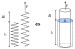
\includegraphics[scale=1]{../Figures_chap_intro/hooke.pdf}
\caption[Loi de Hooke pour un ressort]{Déformations d'un solide induites par une force extérieure. Tout solide élastique se comporte comme un ressort dont la raideur dépend de son module d'Young $E$ et de sa géométrie.}
\end{figure}


\newpage
%
%Lorsqu'un ressort idéal de longueur $l$ est soumis à une force de traction ou de compression, celui-ci se déforme, et produit une force $\vec{F}$ dans la direction opposée à la déformation en retour. Cette force est proportionnelle à l'étirement du ressort $\Delta l$, selon un coefficient de raideur $k$ de telle sorte que
%
%\begin{equation}
%F=-k\Delta l
%\end{equation}
%
%Le modèle du ressort décrit une pièce mécanique idéalisée, que l'on ne déformerait que selon un seul axe, et qui n'aurait qu'une seule dimension. Cette pièce se comporte alors comme un ressort, dont la longueur et la raideur sont déterminées par les propriétés du matériau qui la compose et sa géométrie. La loi de Hooke est une généralisation de la loi des ressors pour un solide.
%

\subsubsection{Loi de Hooke uniaxiale pour un solide élastique}

\myparagraph{Module d'Young}

%La géométrie d'une pièce mécanique est un facteur déterminant de sa réponse aux contraintes extérieures.
Lorsqu'une pièce mécanique est soumise à une force extérieure, l'étirement total qu'elle subit dépend de sa géométrie. À force égale, une barre deux fois plus longue s'allonge deux fois plus, tandis que la même force appliquée sur une surface deux fois plus grande l'allonge deux fois moins. Afin d'éliminer ces considérations, nous utilisons la contrainte $\sigma=F/A$ définie comme le rapport de la force $F$ appliquée sur la surface $A$, et l'allongement relatif, ou déformation, $\varepsilon=\Delta l/l_0$ défini comme le rapport entre l'allongement de la pièce $\Delta l$ et sa longueur à vide $l_0$. La \textit{loi de Hooke}\,\cite{hooke_potentia_1674} stipule alors qu'il existe un coefficient $E$ nommé \textit{module d'Young} tel que

\begin{equation}
\sigma=E\varepsilon
\end{equation}

Cette pièce se comporte alors comme un ressort, dont la raideur est déterminée par les propriétés du matériau qui la compose, sa longueur et sa géométrie. La loi de Hooke est une généralisation de la loi des ressorts pour un solide. Le module d'Young s'exprime en pascals. Pour le PMMA, matériau que nous utilisons dans cette étude, $E_{PMMA}\sim\SI{3}{\giga\pascal}$.
%et sa valeur varie typiquement du mégapascal pour les matériaux tels que le caoutchouc à plusieurs centaines de gigapascals pour les métaux\,\cite{feynman_feynman_1963}.

\myparagraph{Coefficient de Poisson}

La pièce raccourcie ou allongée sous l'effet de la contrainte voit également sa largeur changer. Lorsqu'un matériau est soumis à une contrainte $\sigma_\parallel$ selon un axe, il subit une déformation $\varepsilon_{\parallel} =\sigma_{\parallel} /E$ selon cet axe, mais également une déformation $\varepsilon_\perp$ dans le plan orthogonal à cet axe. Le \textit{coefficient de Poisson} est alors défini comme


\begin{equation}
\nu = -\frac{\varepsilon_\perp}{\varepsilon_{\parallel} }
\end{equation}


Le coefficient de Poisson est sans unité. Il prend des valeurs entre 0 et 0.5 et varie typiquement de 0.1 à 0.4 dans la plupart des matériaux courants\,\cite{feynman_feynman_1963}.

\subsubsection{Loi de Hooke généralisée}

Si l'on s'intéresse maintenant à une contrainte non unidirectionnelle, les contributions des contraintes s'additionnent. Il nous faut considérer le cas d'un petit cube de matière infinitésimal soumis à des contraintes, exprimées sous la forme d'un tenseur $[\sigma] = [\sigma_{i,j}]_{i,j\in\{1,2,3\}}$, où 1, 2 et 3 représentent les trois directions d'un repère orthonormé. Il en va de même pour $[\varepsilon]$. Sous l'hypothèse que le matériau est homogène et isotrope, toujours vérifiée par la suite, la loi de Hooke se généralise\,\cite{feynman_feynman_1963} sous la forme

\begin{equation}
[\sigma] = \frac{E}{1+\nu }\left( [\varepsilon] +\frac{\nu }{1-2\nu }\operatorname{Tr}\left( [\varepsilon] \right) \mathbf I_3 \right) 
\end{equation}

Soit encore en convention de sommation d'Einstein

\begin{equation}
\sigma_{ij} = \frac{E}{1+\nu } \left( \varepsilon_{ij}+\frac{\nu }{1-2\nu }\varepsilon_{kk} \delta _{ij}\right)
\end{equation}


Ainsi nous disposons d'une relation close permettant de lier les déformations aux contraintes subies par un matériau. Couplées à des conditions aux limites et des informations sur la géométrie des pièces considérées, cette équation nous permet de résoudre entièrement le problème de la répartition des contraintes. Dans notre étude nous utilisons des pièces dont la forme est celle de plaques minces, qui nous permettent de considérer un système 2D à trois degrés de liberté.


\subsubsection{Cas des plaques}

Une \textit{plaque} est une pièce dont la forme est celle d'un parallélépipède dont une des dimensions, notée $z$, est beaucoup plus faible que les autres. Sous la condition que la pièce est une plaque mince, nous pouvons effectuer l'hypothèse dite de \textit{planéité des contraintes} (\textit{plane stress}), qui considère que les contraintes appliquées selon l'axe $z$ sont toutes nulles, c'est à dire que $\sigma_{xz}=\sigma_{yz}=\sigma_{zz}=0$. Sous cette hypothèse la loi de Hooke se réécrit\,\cite{freund_dynamic_1990}


\begin{equation}
\begin{pmatrix}
\sigma_{xx} \\
\sigma_{yy} \\
\sigma_{xy}
\end{pmatrix}
=
\dfrac{E}{1-\nu^2}\times\begin{pmatrix}
1 & \nu & 0 \\
\nu & 1 & 0 \\
0 & 0 & \frac{1-\nu}{2} 
\end{pmatrix}
\cdot
\begin{pmatrix}
\varepsilon_{xx} \\
\varepsilon_{yy} \\
\varepsilon_{xy}
\end{pmatrix}
\end{equation}


Ainsi dans le cas de plaques minces telles que celles que nous étudions, nous pouvons restreindre l'étude des déformations du matériau à trois composantes indépendantes. Nous nous placerons par la suite dans le cadre de plaques minces disposées dans le plan $(x,y)$.

Une autre hypothèse de planéité est possible, celle de planéité des déformations (\textit{plane strain}), que nous ne considérerons pas dans cette étude.


\subsection{Théorie de la fracture linéaire élastique (LEFM)}

Lorsqu'un matériau est étiré jusqu'au point de se briser, l'énergie qu'il faut lui apporter pour causer sa rupture peut à première vue s'apparenter à celle nécessaire pour briser des liaisons atomiques ou moléculaires en son sein. Pourtant le verre se brise lorsqu'il est soumis à une contrainte de l'ordre de \SI{100}{\mega\pascal}, alors que la rupture de ses liaisons nécessiterait une contrainte 100 fois supérieure. C'est pour résoudre ce paradoxe que l'ingénieur aéronautique anglais A.\,A.\,Griffith a développé lors de la Première Guerre Mondiale la mécanique de la fracture. Il s'agit du domaine de la physique étudiant la création et la propagation des fissures au sein des matériaux, ainsi que la réponse des matériaux à ces fissures. Ses applications vont de la recherche fondamentale à l'ingénierie pratique, en raison de l'omniprésence des fractures, objets principaux de cette section, au sein des matériaux.

Sauf précision contraire, nous considérons que les fractures étudiées sont statiques ou quasi-statiques, sous un chargement constant appliqué à grande distance de la fissure.


\subsubsection{Qu'est-ce qu'une fracture ?}
\begin{figure}[htb]
\centering
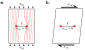
\includegraphics[scale=1]{../Figures_chap_article/crack_griffith.pdf}
\caption[Concentration des contraintes en pointe de fissure]{Représentation schématique de deux fractures. \textbf{a.}\,Fracture de longueur $\ell$ en mode d'ouverture. Une contrainte d'étirement $\sigma_{yy}$ homogène est appliquée au système. Les lignes rouges représentent les lignes de force dans le matériau. Une concentration des lignes de force indique une augmentation de la contrainte locale\,\cite{ohring_engineering_1995}. \textbf{b.}\,Fracture de longueur $\ell$ en mode de cisaillement dans le plan. Une contrainte de cisaillement $\sigma_{xy}$ homogène est appliquée au système. Les cercles rouges indiquent une concentration des contraintes.}
\label{fig:griffith_intro}
\end{figure}




Lorsqu'une contrainte $\sigma$ est appliquée aux bords d'un matériau élastique isotrope, elle est transmise à l'intérieur de celui-ci selon la loi de Hooke. Si le milieu est homogène, chaque volume infinitésimal du matériau supporte la même contrainte, mais si un défaut apparaît, il peut être le siège d'une concentration des contraintes, ce qui en fait un point de faiblesse du matériau. Une \textit{fracture}, ou \textit{crack}, ou encore \textit{rupture}, est un défaut du matériau consistant en une surface le long de laquelle les contraintes sont nulles.

Un exemple de fracture dans un matériau soumis à une contrainte d'extension est une déchirure dans une feuille mince que l'on étire (Fig.\,\ref{fig:griffith_intro}a). Lors de l'étirement de la feuille, les bords de la déchirure ne supportent aucune contrainte $\sigma_{yy}$. Sa pointe en revanche accumule de plus grandes contraintes que le reste du matériau, ce qui mène à terme à sa propagation, et à la déchirure complète de la feuille. C'est par l'existence de ce type de fractures que Griffith a répondu à la question initiale de son étude portant sur les fibres de verre. Les microfissures dans le verre, dues aux imperfections de fabrication, mènent à une accumulation de contraintes et à la rupture précoce de l'échantillon\,\cite{griffith_phenomena_1921}.












\subsubsection{Critère d'initiation de Griffith}


Si une fracture est présente dans un matériau au repos, elle ne se propage pas. Lorsque le matériau est chargé et la contrainte appliquée à l'interface est suffisante, la fracture peut s'étendre. Cette contrainte limite $\sigma_c$ dépend des propriétés du matériau, mais également de la longueur de la fracture. Afin de la déterminer il nous faut effectuer un bilan d'énergie. Deux énergies sont en jeu dans la propagation d'une fracture. La première est l'énergie potentielle élastique stockée par le matériau en raison des déformations. L'énergie potentielle élastique totale du matériau $E_{el}$ s'exprime grâce à la densité d'énergie potentielle locale $e_{el}$ par

\begin{equation}
E_{el} = \iiint e_{el}\,\mathrm{d}\mathcal{V}\qquad\text{avec}\qquad e_{el}=\frac{1}{2}\varepsilon\cdot\sigma
\end{equation}


Dans un matériau contenant une fracture, celle-ci créé une ligne de contraintes nulles, et relâche une partie de cette énergie par rapport au matériau sans défaut. L'énergie relâchée par unité de longueur du crack est notée $W$. Nous définissons $G=-\partial W/\partial\ell$ le \textit{taux de restitution d'énergie} (\textit{energy release rate}) correspondant à l'énergie libérée par la propagation de la fracture par unité de longueur. Il nous faut ensuite considérer l'énergie nécessaire à la création du défaut par unité de longueur, notée $U$. La fracture ne peut se propager que lorsque les variations de ces deux énergies linéiques avec la longueur du crack $\ell$ se compensent. Le critère de Griffith est alors que l'énergie libérée par le relâchement élastique compense l'énergie nécessaire à la création des surfaces libres, soit

\begin{equation}
\dfrac{\partial\:}{\partial\ell}\left(W-U\right)=0
\end{equation}

Dans son article fondateur Griffith considère le cas d'une plaque mince contenant une fissure de le longueur $\ell$ et soumise à une contrainte en ouverture $\sigma$ uniforme et constante, dans l'hypothèse de planéité des contraintes\,\cite{griffith_phenomena_1921}. Il montre alors que

\begin{equation}
W\propto \ell^2\sigma^2/E
\end{equation}

De plus l'énergie $U$ peut s'exprimer en fonction de la longueur de la fissure à l'aide de \textit{l'énergie de fracture} $\Gamma$, qui est une caractéristique du matériau, sous la forme

\begin{equation}
U = \Gamma \ell
\end{equation}

Ainsi le critère de Griffith devient

\begin{equation}
G=\Gamma
\end{equation}


Cette équation permet d'établir l'expression d'une contrainte limite $\sigma_c$ à partir de laquelle la fracture se propage\,\cite{griffith_phenomena_1921,freund_dynamic_1990}

\begin{equation}
\sigma_c\propto\sqrt{\frac{\Gamma E}{\ell}}
\end{equation}

Ainsi la contrainte $\sigma_c$ nécessaire pour déstabiliser une fracture est une grandeur décroissante de la longueur de celle-ci. La valeur exacte de cette contrainte dépend de la géométrie considérée. Dans le cas d'un système de taille infinie avec un chargement homogène en ouverture\,\cite{sun_fracture_2012}


\begin{equation}
\sigma_c=\sqrt{\frac{\Gamma E}{\pi\ell(1-\nu^2)}}
\end{equation}


Il est possible de considérer $\Gamma$ comme la valeur critique de $G$, notée également $G_c = \Gamma$. Conjointement la longueur de Griffith est définie comme la longueur critique $\ell_c\propto1/\sigma^{2}$ telle que $G=\Gamma$.


Ce critère nous permet de déterminer le point critique pour lequel la fracture s'initie, mais ne nous renseigne pas sur la forme que prennent les contraintes à son passage. Les contributions de G.\,R.\,Irwin et M.\,L.\,Williams (1957)\,\cite{irwin_analysis_1957,williams_stress_1957} ont éclairé ce point, et nous permettent de déterminer la forme du tenseur des contraintes au voisinage de la fracture, et en particulier à sa pointe.






\subsubsection{Facteur d'intensité des contraintes}
\begin{figure}[htb]
\centering

\includegraphics[scale=1]{../Figures_chap_intro/polaire.pdf}
\caption[Coordonnées polaires]{Définition des coordonnées polaires dans le cadre de la propagation d'une fracture. Le repère généralement utilisé pour décrire une fracture est solidaire de sa pointe, définissant $r$ comme la distance à celle-ci et $\theta$ l'angle par rapport à la direction de propagation.}
\label{fig:polaire}
\end{figure}


Lorsqu'un matériau contient une fissure, les tenseurs des contraintes et déformations en son sein sont altérés. En effet les coins de la fissure concentrent de fortes contraintes, tandis qu'elles sont nulles le long de la fissure. Dans le cadre de l'étude d'un solide idéalement élastique et linéaire il est possible de déterminer leur expression à proximité de la pointe de la fissure\,\cite{irwin_analysis_1957,williams_stress_1957,erdogan_fracture_2000,sun_fracture_2012}.


Nous repérons la position d'un point dans le matériau par ses coordonnées polaires $(r,\theta)$ par rapport à la pointe de la fissure (Fig.\,\ref{fig:polaire}). La résolution des équations de l'élasticité sous les hypothèses considérées donne l'expression générale du tenseur $\sigma_{ij}$ en un point $(r,\theta)$ sous la forme d'un développement en séries de Williams\,\cite{williams_stress_1957} comme suit, où les fonctions $g_{ij}^n$ sont des fonctions angulaires connues

\begin{equation}
\sigma_{ij}=\sum_{n=-1}^{+\infty} A_n\,r^{n+1/2}\,g^n_{ij}(\theta)
\end{equation}

Ce développement en puissances de $r$ ne prend que des valeurs demi-entières. Il commence en $n=-1$ pour satisfaire la convergence de l'énergie en pointe de fissure. Pour le montrer nous nous plaçons dans les coordonnées cylindriques, $\mathrm{d}\mathcal{V}(r)=r\mathrm{d\theta}\,\mathrm{d}r\,\mathrm{d}z$. Si nous considérons un des termes $\sigma = r^{\lambda}$ du développement, l'énergie élastique associée contenue en pointe de fissure dans un cercle de rayon $r$ est

\begin{equation}
\begin{aligned}
W(r)&=\frac{1}{2}\iiint\sigma\cdot\varepsilon\,\mathrm{d}\mathcal{V}(r)\propto \int_{0}^r \rho_r^{2\lambda+1}\,\mathrm{d}\rho_r
\end{aligned}
\end{equation}

Ainsi l'énergie contenue en pointe de fissure ne converge donc que si $\lambda > -1$.

À grande distance de la pointe de fissure, le tenseur des contraintes est régi par les termes tels que $n\geq0$. Cependant à proximité de la pointe, le terme en $n=-1$ diverge, et domine donc tous les autres. Par conséquent l'expression des contraintes en pointe de fissure peut être donnée par le développement limité suivant\,\cite{sun_fracture_2012}

\begin{equation}
\sigma_{ij} = \frac{K}{\sqrt{2\pi r}}f_{ij}(\theta)+\Theta\left(r^{1/2},r^{3/2},\dots\right)
\label{eq:joceline}
\end{equation}

Dans cette équation les $f_{ij}=g_{i,j}^{n=-1}$ sont des fonctions universelles dont l'expression est ·connue, et $K$ est nommé \textit{facteur d'intensité des contraintes}. Cette quantité, dont la valeur dépend de la géométrie du système et du chargement, fixe l'amplitude des contraintes subies par la pointe de fissure. Il est possible de reformuler le critère de Griffith en termes de facteur d'intensité des contraintes en définissant $K_c\sim\sqrt{\Gamma E}$ la \textit{ténacité} d'un matériau comme la valeur de $K$ lorsque $\sigma=\sigma_c$\,\cite{irwin_analysis_1957}. Cette valeur est une caractéristique du matériau. Pour le PMMA, $K_c\simeq\SI{1.1}{\mega\pascal\meter\tothe{1/2}}$\,\cite{ohring_engineering_1995}.

Le facteur d'intensité de contraintes $K$ prend la forme du produit de la contrainte à grande distance du crack et d'un facteur géométrique dépendant de la longueur du crack, il est donc possible de le calculer pour des géométries simples. Dans le cas général le calcul peut se décomposer par linéarité en un jeu de trois équations indépendantes selon des modes, comme présenté dans la section suivante.

Lorsque la contrainte atteint la limite de plasticité du matériau $\sigma_Y$ (Fig.\,\ref{fig:yield}), les déformations ne peuvent plus être considérées comme élastiques. La zone dans laquelle l'expression obtenue avec l'hypothèse d'élasticité n'est plus valable est nommée \textit{zone de régularisation des contraintes} (\textit{process zone}). Les considérations énergétiques associées aux phénomènes non-linéaires ayant lieu dans cette zone sont incorporées dans une définition plus générale de l'énergie de fracture.



\subsubsection{Modes de fracture}


\begin{figure}[htb]
\centering
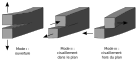
\includegraphics[scale=1]{../Figures_chap_intro/modes.pdf}
\caption[Modes de fracture]{Représentation des trois modes de fracture. Chaque mode évolue indépendamment des deux autres, ce qui permet de décomposer la solution générale des équations de la mécanique de la fracture linéaire élastique sur chacun d'eux.}
\label{fig:modes}
\end{figure}


Les fractures peuvent être décomposées en 3 modes selon le mode de chargement, c'est à dire la direction des contraintes appliquées relativement à leur direction de propagation\,\cite{freund_dynamic_1990,sun_fracture_2012} (Fig.\,\ref{fig:modes}). La fracture en ouverture est dite de \textit{mode\:\textsc{i}}, la contrainte nulle le long de la fracture est $\sigma_{yy}$. La contrainte nulle le long d'une fracture en cisaillement dans le plan, dite de \textit{mode\:\textsc{ii}}, est la contrainte cisaillante $\sigma_{xy}$. Le mode\:\textsc{iii} pour sa part correspond à un cisaillement hors du plan de propagation de la fracture. Il se caractérise par le fait que seuls les $\sigma_{zj}$ ne sont pas nuls partout. Dans le cadre de la fracture linéaire, en raison de la linéarité, ces trois modes peuvent être étudiés indépendamment, leurs contributions sont alors superposées pour décrire une fracture en mode mixte.

\newpage

Ainsi il est possible de décomposer $[\sigma]$ selon chacun de ces modes

\begin{equation}
[\sigma]=\sum_{\textsc{m}=\textsc{i,ii,iii}}[\sigma^\textsc{m}]
\end{equation}


Nous pouvons ensuite définir un facteur d'intensité des contraintes $K_\textsc{m}$ pour chaque mode puis décomposer l'Équation\,\ref{eq:joceline} comme

\begin{equation}
\sigma_{ij} = 
\sum_{\textsc{m}\in\{\textsc{i,ii,iii}\}}
\sigma_{ij}^\textsc{m}
\quad\text{avec}\quad
\sigma_{ij}^\textsc{m}=
\frac{K_\textsc{m}}{\sqrt{2\pi r}}f_{ij}^\textsc{m}(\theta)+\Theta\left(r^{1/2},r^{3/2},\dots\right)
\label{eq:sigmamodes}
\end{equation}




Les expressions des fonctions $f_{ij}^\textsc{m}$ sont alors les suivantes\,\cite{sun_fracture_2012}



\begin{equation}
\resizebox{150mm}{!}{
$
\begin{cases}
	f^\textsc{i}_{xx}&=\left(1-\sin\frac{\theta}{2}\,\sin\frac{3\theta}{2} \right)\cos\frac{\theta}{2}\\[.5em]
	f^\textsc{i}_{yy}&=\left(1+\sin\frac{\theta}{2}\,\sin\frac{3\theta}{2} \right)\cos\frac{\theta}{2}\\[.5em]
	f^\textsc{i}_{xy}&=\sin\frac{\theta}{2}\,\cos\frac{3\theta}{2}\,\cos\frac{\theta}{2}
\end{cases}
\quad
\begin{cases}
	f^\textsc{ii}_{xx}&=-\left(2+\cos\frac{\theta}{2}\,\cos\frac{3\theta}{2}\right)\sin\frac{\theta}{2}\\[.5em]
	f^\textsc{ii}_{yy}&=\cos\frac{\theta}{2}\,\cos\frac{3\theta}{2}\,\sin\frac{\theta}{2}\\[.5em]
	f^\textsc{ii}_{xy}&=\left(1-\sin\frac{\theta}{2}\,\sin\frac{3\theta}{2} \right)\cos\frac{\theta}{2}
\end{cases}
\quad
\begin{cases}
	f^\textsc{iii}_{zx}&=-\sin\frac{\theta}{2}\\[.5em]
	f^\textsc{iii}_{zy}&=\cos\frac{\theta}{2}\\
\end{cases}
$}
\end{equation}

L'expression de $f_{zz}^{\textsc{i},\textsc{ii}}$ dépend de l'hypothèse de planéité choisie
\begin{equation}
f_{zz}^{\textsc{i},\textsc{ii}}=
\begin{cases}
0&\quad\text{planéité des contraintes}\\
\nu(f_{xx}+f_{yy})&\quad\text{planéité des déformations}
\end{cases}
\end{equation}


L'expression des fonctions $f^\textsc{m}_{ij}$ en $\theta=0$ permet de donner une expression des $K_\textsc{m}$ permettant notamment leur mesure :

\begin{equation}
\begin{aligned}
K_\textsc{i}&=\lim_{\:r\rightarrow 0^+}\sqrt{2\pi r}\;\sigma_{yy}(r,\theta=0)\\
K_\textsc{ii}&=\lim_{\:r\rightarrow 0^+}\sqrt{2\pi r}\;\sigma_{xy}(r,\theta=0)\\
K_\textsc{iii}&=\lim_{\:r\rightarrow 0^+}\sqrt{2\pi r}\;\sigma_{zy}(r,\theta=0)
\end{aligned}
\end{equation}


La séparation de l'Équation\,\ref{eq:joceline} en modes indépendants permet également de définir des valeurs de $G$ par mode, notées $G_\textsc{m}$. L'expression complète de $G$ est alors donnée par
\begin{equation}
G=\frac{1-\nu^2}{E}\left(K_\textsc{i}^2+K_\textsc{ii}^2\right) + \frac{1+\nu}{E}K_\textsc{iii}^2
\end{equation}






\begin{figure}[p]
\centering
\begin{tabular}{lccc}
Matériau & $\Gamma\left(\mathrm{kJ.m}^{-2}\right)$ & $K_{I c}\left(\unit{\mega\pascal\meter\tothe{1/2}}\right)$ & $E(\mathrm{GPa})$ \\
\hline & & & \\
Acier allié & 107 & 150 & 210 \\
Aluminium allié & 20 & 37 & 69 \\
Acier & 12 & 50 & 210 \\
Caoutchouc & 13 & - & 0.001 \\
époxy & 2 & 2.2 & 2.4 \\
PMMA & 0.5 & 1.1 & 2.5 \\
Polystyrène & 0.4 & 1.1 & 3 \\
Bois & 0.12 & 0.5 & 2.1 \\
Verre & 0.007 & 0.7 & 70 \\
\hline
\end{tabular}
\caption[Caractéristiques de différents matériaux]{Caractéristiques de différents matériaux pour une fracture en mode\:\textsc{i} (extrait de\,\cite{ohring_engineering_1995}). Il est possible de montrer que $\Gamma\simeq K^2/E$.}
\label{tab:caracmater}
\end{figure}


\begin{figure}[p]
\centering
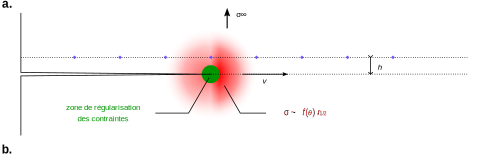
\includegraphics[scale=1]{../Figures_chap_intro/LEFM_plot_mesure.pdf}
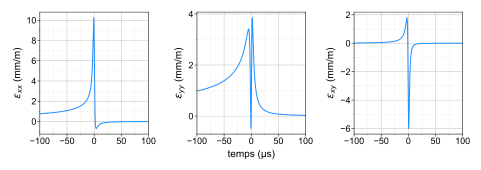
\includegraphics[scale=1]{../Figures_chap_intro/LEFM_plot.pdf}
\caption[Simulation d'une rupture dynamique en mode \textsc{i}]{\textbf{a.}\,Propagation et mesure d'une rupture en mode\:\textsc{i}. La rupture se propage le long de la ligne pointillée du bas à une vitesse $v$. Les capteurs de déformation mesurant $\varepsilon$ sont disposés le long de la ligne pointillée du haut, à une distance $h$ de la ligne de propagation de la rupture. Afin de mesurer le passage de la rupture et sa forme caractéristique, la distance $h$ doit être choisie supérieure au rayon de la zone de régularisation mais dans la zone où le terme en $\sigma\sim r^{-1/2}$ domine le développement en série de Williams. \textbf{b.}\,Évolution de $\varepsilon$ en fonction du temps au passage d'une fracture à $h=\SI{1}{\milli\meter}$ du point de mesure. L'oscillation en vaguelette observée est la signature de la fonction angulaire $\Sigma_{ij}^\textsc{m}$. La fracture se déplace à $v=\SI{500}{\meter\per\second}$, et l'énergie de fracture du matériau est $G=\SI{2}{\kilo\joule\per\meter\squared}$ (similaire à du PMMA).}
\label{fig:simulfrac}
\end{figure}








En résumé, nous avons vu qu'au sein d'un matériau, la pointe d'une rupture statique ou quasi-statique de longueur $\ell$ est le siège d'une concentration des contraintes. Le critère d'initiation de rupture de Griffith indique que lorsque le taux de restitution d'énergie $G$ est égal à l'énergie de fracture du matériau $\Gamma$ (Fig.\,\ref{tab:caracmater}), la fracture peut se propager, permettant la définition d'une contrainte limite $\sigma_c$ pour une rupture de longueur $\ell$. Cette contrainte s'exprime comme $\sigma_c\propto\sqrt{\Gamma E/\ell}$, le facteur de proportionnalité dépendant de la géométrie considérée. La contrainte en pointe de fissure s'exprime comme une série de Williams dont le terme dominant à proximité de la pointe de fissure est $\sigma\propto K/\sqrt{r}$, avec $K$ le facteur d'intensité des contraintes, qui lorsque la contrainte atteint $\sigma_c$ vaut $K = K_c$ la ténacité du matériau (Fig.\,\ref{tab:caracmater}). Nous avons enfin vu qu'il était possible de décrire tout crack comme la superposition de trois modes indépendants par linéarité. Cette séparation permet notamment de redéfinir les caractéristiques du matériau et critère d'initiation par mode.

Les trois modes ont leur propre critère d'initiation, et leur équation de propagation. L'évolution de la rupture est alors décrite par les lois de la fracture dynamique.


\subsection{Fracture dynamique}





Une fois déstabilisée, une rupture peut se propager dynamiquement dans le matériau. Si sa vitesse $v$ est telle que $v<c_r$ la vitesse des ondes de Rayleigh dans le matériau, la rupture est dite \textit{sub-Rayleigh}. Elle est alors décrite par la mécanique de la fracture linéaire élastique. Si cependant elle se déplace à $v>c_s$ la vitesse des ondes de cisaillement, elle est dite \textit{supershear}. Dans ce cas, la convergence du flux d'énergie élastique en point de fissure ne permet pas d'expliquer sa propagation, qui dépend d'un cadre physique différent\,\cite{dunham_supershear_2003}.

\subsubsection{Expression du tenseur des contraintes}


Dans le cas des ruptures sub-Rayleigh sous un chargement constant, l'expression de $\sigma_{ij}^\textsc{m}$ dépend de la vitesse, et en particulier des rapports $\alpha_s =\sqrt{ 1-(v/c_s)^2}$ et $\alpha_p =\sqrt{ 1-(v/c_p)^2}$ où $c_p$ et $c_s$ sont les vitesses des ondes de compression et de cisaillement dans le matériau. L'expression des facteurs d'intensité des contraintes est alors donnée par

\begin{equation}
K_\textsc{m}(v)=K_\textsc{m}^S\times k_\textsc{m}^d(v)
\end{equation}

Dans cette expression $K_\textsc{m}^S = K_\textsc{m}(v=0)$ correspond au facteur d'intensité des contraintes statique ou quasi-statique, et $k_\textsc{m}^d(v)$ est une fonction connue de la vitesse de propagation. Cette expression n'est valide que pour un système quasi-infini, pour lequel les ondes émises par la rupture n'ont pas eu le temps de se réfléchir sur un bord. Sous cette hypothèse il est possible de calculer $K_\textsc{m}(v)$.

Les fonction $f_{ij}^\textsc{m}(\theta)$ dans l'Équation\,\ref{eq:sigmamodes} sont également remplacées par des fonctions dynamiques $\Sigma_{ij}^\textsc{m}(\theta,v)$ connues, exhibant en modes \textsc{i} et \textsc{ii} une divergence lorsque $v\rightarrow c_r$, et lorsque $v\rightarrow c_s$ en mode \textsc{iii}. L'expression du tenseur des contraintes en pointe de fissure est alors donnée par\,\cite{sun_fracture_2012}


\begin{equation}
\sigma_{ij}^\textsc{m}=\frac{K_\textsc{m}^Sk^d_\textsc{m}(v)}{\sqrt{2\pi r}}\Sigma^\textsc{m}_{ij}(\theta,v)+\Theta(r^{1/2},r^{3/2},\dots)
\label{eq:sigmamodedyn}
\end{equation}

Lors du passage d'une rupture à proximité d'un capteur de déformation, la coordonnée $\theta$ repérant le point de mesure dans le référentiel de la pointe de fissure passe de $\theta\rightarrow\SI{0}{\degree}$ à $\theta\rightarrow\SI{180}{\degree}$. Ainsi la mesure balaie la fonction angulaire $\Sigma_{ij}^\textsc{m}$ et exhibe une variation caractéristique en vaguelette (Fig.\,\ref{fig:simulfrac}). La mesure de $\varepsilon$ au passage de la rupture permet de déterminer $\Gamma$ par un ajustement\,\cite{svetlizky_brittle_2019}.

\newpage


\subsubsection{Critère de propagation}

Le critère de propagation d'une rupture dynamique est identique au critère d'initiation d'une rupture statique, c'est à dire que le taux de restitution d'énergie $G$ doit être égal à l'énergie de fracture $\Gamma$, mais $G$ dépend de la vitesse de propagation. Il est possible d'exprimer $G$ sous la forme

\begin{equation}
G(v)\propto\frac{K^2}{E}\times A(v)\quad\text{et}\quad G(v) = \Gamma
\label{eq:propagfracdyn}
\end{equation}

La fonction $A(v)$, nommée facteur dynamique, prend en mode\:\textsc{i} et \textsc{ii} la forme

\begin{equation}
A(v)=\dfrac{\alpha_p(1-\alpha_s^2)}{4\alpha_p\alpha_s-(1+\alpha_p^2)^2}
\end{equation}

Ce facteur diverge lorsque $v\rightarrow c_r$ la vitesse des ondes de Rayleigh, correspondant à la première racine réelle du dénominateur de $A(v)$. Cette égalité indique que l'énergie nécessaire à la propagation d'une rupture sub-Rayleigh en mode\:\textsc{i} ou \textsc{ii} diverge lorsque la vitesse de propagation approche $c_r$, ce qui en fait la vitesse maximale de ce type de rupture. Pour une rupture en mode\:\textsc{iii} la vitesse limite est $c_s$.






\subsection{Fracture frictionnelle}
\label{sec:LEFMfric}



Pour décrire la mise en glissement d'une interface frictionnelle,
l'extension spatiale de celle-ci doit être considérée, contrairement à l'approche adoptée dans les modèles Rate-and-State, qui décrivent le mouvement du centre de masse du système
(Sec.\,\ref{sec:rateandstate}). En effet cette initiation du mouvement est due à un affaiblissement de l'interface par un front propagatif qui peut s'assimiler à un front de rupture. Il a été montré que ce front est une fracture en mode de cisaillement décrite par la mécanique de la fracture linéaire élastique\,\cite{svetlizky_brittle_2019}. Dans cette section nous présentons les spécificités théoriques de la fracture frictionnelle.


\subsubsection{Phénoménologie}

Une rupture fragile classique amorcée en un point de l'espace se propage dans le matériau alentour en raison de l'accumulation des contraintes en sa pointe, rompant le bloc le long de sa trajectoire. Dans le cas d'une rupture frictionnelle, l'interface est pressée et chargée à grande distance et accumule des contraintes cisaillantes. La rupture peut alors nucléer en un point de l'interface où un microcontact atteint sa résistance au cisaillement, se rompt et se met en glissement (Sec.\,\ref{sec:microfric}). Cette mise en glissement reporte les contraintes que le contact portait sur les aspérités avoisinantes, rompant de proche en proche ces microcontacts le long de l'interface. La rupture peut se propager ainsi tout le long de l'interface, jusqu'à avoir affaibli tous les contacts, permettant le glissement inertiel des blocs. Ces ruptures, comme les ruptures en mode de cisaillement classique, se propagent à des vitesses $v$ telles que $v<c_r$ la vitesse des ondes de Rayleigh dans le matériau, ou telles que $v>c_s$ la vitesse des ondes de cisaillement.

Le mouvement de glissement macroscopique des deux blocs est un mouvement inertiel, il ne commence qu'après que la rupture a traversé l'interface entière. Lorsque les blocs ont relâché une quantité suffisante des contraintes cisaillantes, le glissement s'arrête et les microcontacts se reforment (Sec.\,\ref{sec:evolutionmacro}). L'interface peut alors se recharger, et entrer par exemple dans un cycle de stick-slip, pour lequel chaque évènement de slip est initié par une rupture.

Nous présentons dans la section suivante que la propagation de ces ruptures est régie par la mécanique de la fracture.


\subsubsection{Description par la mécanique de la fracture}

La fracture frictionnelle est une fracture en mode\:\textsc{ii}, guidée par un plan faible formé par l'interface. Ce guidage est une composante essentielle de sa propagation, car dans un solide intact, une fracture initiée en mode\:\textsc{ii} est instable, et évolue spontanément vers le mode\:\textsc{i}. Le long de l'interface frictionnelle, l'énergie de fracture associée à l'affaiblissement des microcontacts $\Gamma_\textsc{fric}$ est beaucoup plus faible que celle associée à une fracture du matériau intact $\Gamma_\textsc{bulk}$. Guidée par l'interface, la rupture peut être repérée par la coordonnée $x(t)$ de son front, et il n'est pas exclu que $\Gamma_\textsc{fric}$ dépende de $x$. Ainsi à partir de l'Équation\,\ref{eq:propagfracdyn} nous pouvons écrire

\begin{equation}
\Gamma_\textsc{bulk} \gg \Gamma_\textsc{fric}
\quad\text{et}\quad
G_\textsc{ii}(v) = \Gamma_\textsc{fric}(x)
\end{equation}


Une différence majeure entre une fracture classique et une rupture frictionnelle est que la rupture frictionnelle n'est pas une ligne de contraintes nulles. En effet, là où après le passage d'une rupture classique le matériau est endommagé de manière irréversible, la rupture frictionnelle affaiblit des microcontacts et leur permet de se mettre en mouvement. Les microcontacts supportent toujours après le passage de la rupture une contrainte cisaillante résiduelle $\sigma_{xy} =\sigma_r$ (Sec.\,\ref{sec:microfric}). De plus pour une rupture en mode de cisaillement les contraintes initiales le long de la ligne de propagation de la rupture sont

\begin{equation}
\big[\sigma^\textsc{ii}\big] (\theta = 0,\,r\rightarrow+\infty) = \begin{bmatrix}
0 & \sigma_{xy}^0\\
\sigma_{xy}^0 & 0
\end{bmatrix}
\label{eq:initnormal}
\end{equation}

Ainsi afin de ramener le tenseur des contraintes $[\sigma^\textsc{fric}]$ d'une rupture frictionnelle à celui d'une fracture en mode de cisaillement, la linéarité des équations présentées permet de prendre en compte les conditions initiales par superposition

\begin{equation}
\big[\sigma^\textsc{ii}\big] = 
\big[\sigma^\textsc{fric}\big] -
\begin{bmatrix}
\sigma_{xx}^0 & \sigma_r\\
\sigma_r      & \sigma_{yy}^0
\end{bmatrix}
\label{eq:pmpi}
\end{equation}


Il a de plus été montré que les contraintes divergent en pointe de fissure selon les équations de la mécanique de la fracture linéaire élastique\,\cite{svetlizky_classical_2014}. Elle est dont décrite par l'Équation\,\ref{eq:sigmamodedyn} avec $\textsc{m}=\textsc{ii}$ seulement, c'est à dire





\begin{equation}
\sigma_{ij}^\textsc{fric}
=
\frac
	{K_{\textsc{ii}}(v)}
	{\sqrt{2\pi r}}
\times
	\Sigma_{ij}^{\textsc{ii}}
(\theta,v)
+
\begin{bmatrix}
	\sigma_{xx}^0 & \sigma_r\\
	\sigma_r      & \sigma_{yy}^0
\end{bmatrix}
\label{eq:fracdynfric}
\end{equation}

Dans cette équation $K_\textsc{ii}$ est le facteur d'intensité des contraintes lié à l'énergie de fracture de l'interface frictionnelle $\Gamma = \Gamma_\textsc{fric}$. Cette énergie correspond à l'énergie nécessaire pour affaiblir les microcontacts à l'interface, elle est donc directement liée à l'aire réelle de contact $A_r$, elle-même proportionnelle à $\sigma_{yy}$\,\cite{svetlizky_brittle_2019}. Ainsi

\begin{equation}
\Gamma(x)\propto\sigma_{yy}(x)
\label{eq:homospa}
\end{equation}

Cette rupture frictionnelle a été largement étudiée dans le cas des interfaces solide-solide homogènes, comme présenté dans le Chapitre\:\ref{chap:etatdelart}.

Nous avons au cours de cette section montré que le mouvement de glissement rapide d'une interface frictionnelle est initié par la propagation d'une fracture le long de l'interface. Cette fracture est décrite de manière quantitative par la mécanique de la fracture linéaire élastique. Une question est de savoir si cette description est généralisable à des interfaces complexes comme celles étudiées en mécanique des failles, bien que leur comportement en découle. L'étude de celles-ci est présentée dans la section suivante.

\newpage





